% 
% appendix.tex : part of the Mace toolkit for building distributed systems
% 
% Copyright (c) 2011, Charles Killian, Dejan Kostic, Ryan Braud, James W. Anderson, John Fisher-Ogden, Calvin Hubble, Duy Nguyen, Justin Burke, David Oppenheimer, Amin Vahdat, Adolfo Rodriguez, Sooraj Bhat
% All rights reserved.
% 
% Redistribution and use in source and binary forms, with or without
% modification, are permitted provided that the following conditions are met:
% 
%    * Redistributions of source code must retain the above copyright
%      notice, this list of conditions and the following disclaimer.
%    * Redistributions in binary form must reproduce the above copyright
%      notice, this list of conditions and the following disclaimer in the
%      documentation and/or other materials provided with the distribution.
%    * Neither the names of the contributors, nor their associated universities 
%      or organizations may be used to endorse or promote products derived from
%      this software without specific prior written permission.
% 
% THIS SOFTWARE IS PROVIDED BY THE COPYRIGHT HOLDERS AND CONTRIBUTORS "AS IS"
% AND ANY EXPRESS OR IMPLIED WARRANTIES, INCLUDING, BUT NOT LIMITED TO, THE
% IMPLIED WARRANTIES OF MERCHANTABILITY AND FITNESS FOR A PARTICULAR PURPOSE ARE
% DISCLAIMED. IN NO EVENT SHALL THE COPYRIGHT OWNER OR CONTRIBUTORS BE LIABLE
% FOR ANY DIRECT, INDIRECT, INCIDENTAL, SPECIAL, EXEMPLARY, OR CONSEQUENTIAL
% DAMAGES (INCLUDING, BUT NOT LIMITED TO, PROCUREMENT OF SUBSTITUTE GOODS OR
% SERVICES; LOSS OF USE, DATA, OR PROFITS; OR BUSINESS INTERRUPTION) HOWEVER
% CAUSED AND ON ANY THEORY OF LIABILITY, WHETHER IN CONTRACT, STRICT LIABILITY,
% OR TORT (INCLUDING NEGLIGENCE OR OTHERWISE) ARISING IN ANY WAY OUT OF THE
% USE OF THIS SOFTWARE, EVEN IF ADVISED OF THE POSSIBILITY OF SUCH DAMAGE.
% 
% ----END-OF-LEGAL-STUFF----
\appendix

\section{Directory Structure}
\label{sec:dir-struct}

This section covers the directory structure of Mace.  You should read this section
if you're either can never figure out where a file is in the repository, or if you are
trying to figure out where to put a new file.

At the top level, there are 5 directories in the release.

\begin{description}
\item[lib] The lib directory contains general purpose code with useful interfaces that may be 
            useful in building applications and services.  They include the logging
            facilities, a facility for operating on command-line and file parameters, the Mace
            stl extensions, a variety of Util functions and much more.  An overview of these is
            in \S~\ref{sec:lib}.  This directory should contain code which (a) has no 
            dependencies to other Mace directories, and (b) will be generally useful to more than
            one application, service, or compiler.
\item[perl5] The compiler directory contains the source for compilers
            and a variety of other perl tools.  The primary compiler is
            the \filename{macecc} compiler which operates on \mac files
            and produces C++ source code.  Other compilers here are the
            xmlrpcc compiler generating xmlrpc stubs, and a macemh
            compiler for compiling the service interface files.
\item[services] The services directory contains the interfaces (ServiceClass and Handler definitions) 
            for services, as well as the implementation of various services.  Services by definition
            provide some service class, though they may be a mix of hand-crafted (C++ implemented) and
            generated (via Mace compiler).  The interfaces are all stored in the \directory{services/interfaces}
            directory, without other files there.  (A possible exception is considered for files which
            define things needed by interfaces but for which it does not make sense to place in the 
            \directory{lib} directory.)  The services themselves are stored in the remaining subdirectories.
            Frequently, each directory implements a single service, though it may include supporting files
            or test code in that directory.  Occasionally, however, related services are placed in the 
            same directory.  Note that any \filename{*.cc} in a service directory will be included
            in the directory's library.  The included services and interfaces are covered further in 
            \S~\ref{sec:service-classes} and \S~\ref{sec:packaged-services}.
\item[application] This directory contains the various applications included with Mace.  Some are toy applications
            but most could be made to do useful work with only small modifications.  The applications are
            described in \S~\ref{sec:applications}.  Additionally, there is a \directory{common} subdirectory
            which includes code which is to be shared between applications, as building blocks, but which include
            dependencies in the \directory{services/interfaces} directory, and therefore cannot be included
            as part of the \directory{lib} directory.  Note that to the extent possible, this directory should
            \emph{not} include dependencies on particular services, in an effort to allow this directory to be built 
            without regard for what services are being built.
\item [docs] The files necessary to produce this documentation.  It can be produced by running "make".  To 
            produce it you will need latex and lgrind installed.  For convenience, a pre-built PDF is already
            included.
\end{description}

\section{Service Classes}
\label{sec:service-classes}

%% \begin{figure}[t]
%% \begin{center}
%% 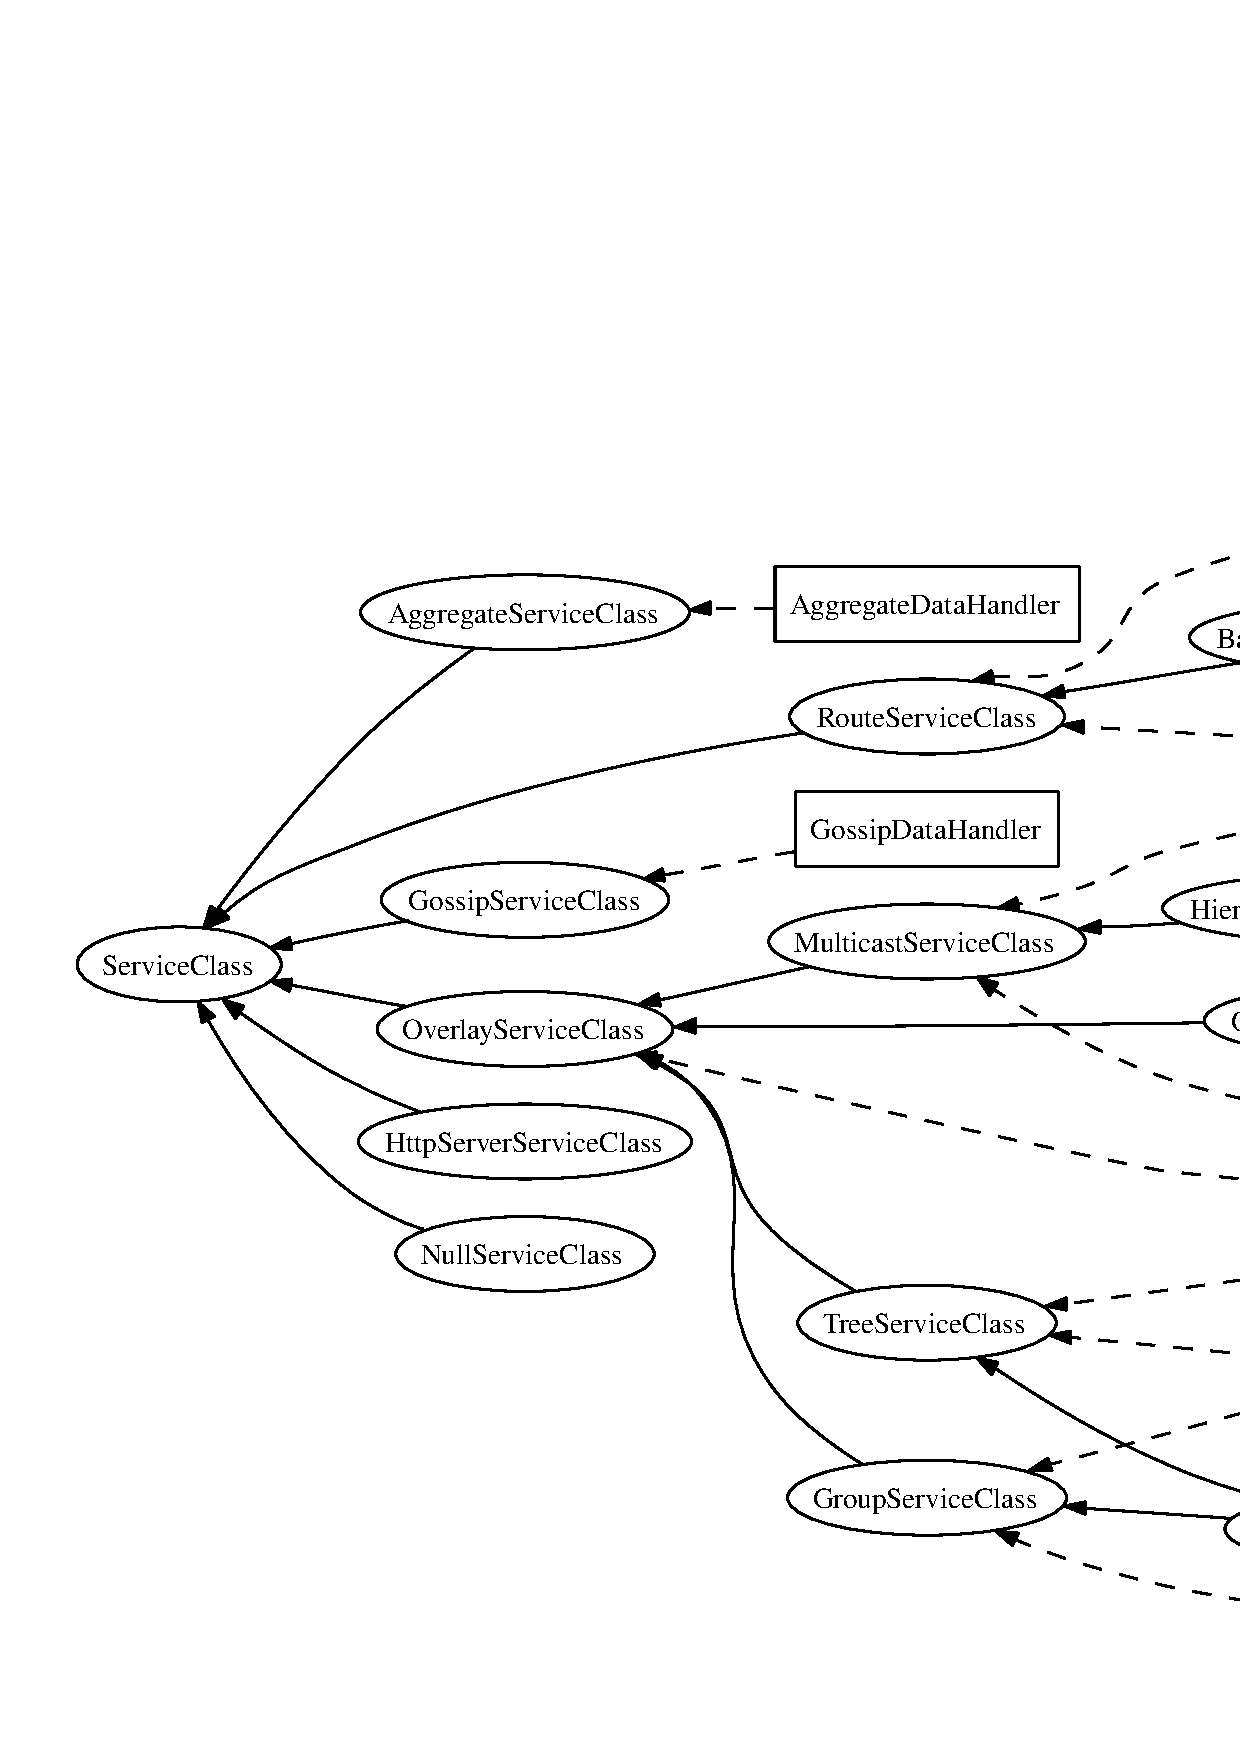
\includegraphics[height=4in]{hierarchy}
%% \caption{\small{Hierarchy of the Mace service classes and
%% handlers.  Service classes are shown in ovals, handlers 
%% in rectangles.  Solid lines indicate inheritance, dashed
%% lines indicate the ``handler'' relationship of a handler
%% to a service class.}}
%% \label{fig:hierarchy}
%% \end{center}
%% \end{figure}

Service classes you will recall define the public interface of a service.
Handlers are interfaces of callback or upcall objects registered with 
a service class.
%%   The structure of the interfaces included with the 
%% present release is described in Figure \ref{fig:hierarchy}.

All service classes derive from the base \typename{ServiceClass}, which 
defines the initialization and de-initialization routines (\function{maceInit}
and \function{maceExit}), respectively.  These functions are special functions
for the Mace compiler: it reference counts them, and recurses them (only once)
to the services used.  It also ensures that the maceInit or maceExit event
only occurs once for the service.

The specific interfaces for each service can best be seen by looking at the 
\filename{.mh} file in the \directory{services/interfaces} directory -- an 
overview of what they contain will be here.

\begin{description}
\item [Sending and Receiving Data] \classname{TransportServiceClass}, \classname{RouteServiceClass}, \classname{MulticastServiceClass},
  and \classname{HierarchicalMulticastServiceClass} define the routing functions found
  in the original MACEDON system.  Each takes a \classname{ReceiveDataHandler} registration for 
  delivery of data.  The primary addition of the \classname{HierarchicalMulticastServiceClass}
  is the \function{collect} and \function{distribute} calls, which transmit data \emph{up} or 
  \emph{down} the hierarchy, respectively.  In the \classname{ReceiveDataHandler} there is a
  \function{forward} call which is performed at all nodes processing the data, including 
  source and destination(s), and a \function{deliver} call, which is called to deliver the data.
  Also related to these services is the \classname{NetworkErrorHandler}, which is used to 
  report node failures, and the \classname{BandwidthRouteServiceClass}, which provides an 
  interface for measuring the bandwidth to a set of peers. which is achieved by the routing.
\item[Aggregation and Gossip] \classname{AggregateServiceClass}, \classname{GossipServiceClass}.
  and their respective handlers are the Mace interfaces for aggregating data and gossiping data.
  Each of these interfaces allows a user to register different aggregations or gossip values for
  different channel ids.
\item[Structures] Service classes have been developed for a few common structures (so far trees
  and overlay routers), to allow shared code for operations over these structures,
  separating out the actual maintenance of the structure.  These service
  classes are \classname{OverlayRouterServiceClass} and
  \classname{TreeServiceClass}.  A special service class presently exists for
  \classname{ScribeTreeServiceClass}, which defines the extra interface
  Scribe-like services provide so they may be managed by SplitStream-like
  services.  This service class will likely have its name changed when it is
  adapted for more general-purpose use.
\item[Overlay and Group] These two service classes define the interface for joining overlays or 
  groups.  They are separated because it is believed that the same interface
  will be useful for different kinds of services, for example joining a
  multicast group or joining a group for threshold cryptography or the
  like\footnote{Similar concepts to groups are starting to appear for
  aggregation, gossip (channel id), or file distribution (file name) -- this
  notion will likely be merged in a future release}.
\item[Http] The Http service class actually provides little interface into it.  It's primary value 
  is the ability to register a handler with the Http service which lets you respond to Http
  queries in Mace-generated code.
\item[Null] The Null service class is one which derives directly from \classname{ServiceClass} and
  provides no additional interface.  Its existance is generally for test code, 
  which is supposed to do its task as a result of \function{maceInit()}.
\end{description}

\section{Packaged Services}
\label{sec:packaged-services}

The following services come pre-implemented in Mace (divided by directory located).

\begin{description}
\item[Transport] Several \classname{TransportServiceClass} services are
  in this directory.  This includes \classname{TcpTransport},
  \classname{UdpTransport}, \classname{MaceTransport} (a user-level
  TCP-like service), \classname{ProvisionalTransport} (which allows
  cancelling messages), and \classname{RouteTransportWrapper} (which
  wraps a \classname{RouteServiceClass} on top of a
  \classname{TransportServiceClass}, providing the forward upcall.)
  Features include built-in encryption and authentication using SSL
  certs, and the ability to run Mace instances using different ports and
  through port-forwarding firewalls or with unroutable nodes.  It also
  stands as the building block for a number of new features we are
  considering.
\item[ReplayTree] \classname{ReplayTree} represents the original MACEDON random tree,
  and provides the \classname{TreeServiceClass} interface by building a tree 
  randomly.  Its random tree features are deprecated by the new \classname{RandTree},
  but it is still useful for constructing a tree by specifying its structure in
  a configuration file (it \emph{replays} a tree determined offline).
\item[RandTree] \classname{RandTree} provides the \classname{TreeServiceClass}
  interface by building a random tree.  Every node joins at the root and finds
  a place in the overlay tree randomly.  This implementation, unlike the MACEDON
  version provides a degree of tolerance for network failures, including root
  failover.
\item[RanSub] This directory contains implementations of \classname{RanSubAggregator},
  an implementation of the \classname{AggregateServiceClass}, and
  \classname{RanSub}, an implementation of the \classname{GossipServiceClass}.
  Unlike a ``standard'' gossip service, \classname{RanSub} provides a uniformly
  random subset of peer data (the gossip) using an aggregation service which
  works simply by passing up and down the tree.
\item[Pastry] This is an implementation of the original Pastry overlay router.
  It does include some degree of recovery from network failures, though it does 
  not include any of the newer Microsoft work on controlling the cost of 
  reliability.  It does provide proximity neighbor selection.
\item[ScribeMS] This is an implementation of the Scribe tree 
  protocol.  The MS refers to the fact that in MACEDON there were two
  implementations of Scribe, one which followed more of the Microsoft design,
  and one which followed more of the Rice design, which have somewhat diverged
  from the original publication.  This release contains several bugfixes as
  compared to the MACEDON implementation.
\item[SplitStreamMS] This is an implementation of the SplitStream forest 
  multicast protocol.  The MS refers to the fact that in MACEDON there were
  two implementations of SplitStream, one which followed more of the Microsoft
  design, and one which followed more of the Rice design, which have somewhat
  diverged from the original publication.  This release contains several bugfixes
  as compared to the MACEDON implementation.
\item[GenericOverlayRoute] This directory contains two implementations of routing over an overlay.
  \classname{RecursiveOverlayRoute} provides basic overlay routing using
  recursive lookups (at each hop, consult with an overlay router to find out
  the next hop).  \classname{CacheRecursiveOverlayRoute} uses recursive routing
  techniques, but establishes direct links to destination nodes for
  applications such as tree multicast which frequently don't want intermediate
  nodes forwarding data between two tree-peers.  It does this transparently
  however so that higher level services need not concern them with the physical
  addresses of the destination nodes but can just refer to them by their overlay
  identifiers.
\item[GenericTreeMulticast] Implements the \classname{HierarchicalMulticastServiceClass}
  given an instance of a \classname{TreeServiceClass} and a \classname{RouteServiceClass}.
  The assumption of this service is that the addressing schemes of these two service
  instances are the same (that nodeids correspond between the two).
\item[Http] Provides an implementation of the \classname{HttpServiceClass},
  with which you may register to receive URL requests matching a certain path.
  May be used either as a service by another service, or as a standalone service.
\item[Chord] This is an implementation of the original Chord overlay router.
\item[DHT] A service for storage in an overlay routed network.
\end{description}

There is effort underway to port services from MACEDON to Mace, and these 
will be included and described as they available.

\section{Logging}
\label{sec:log}
All log messages have selectors and log levels.  Logging can
additionally be enabled or disabled at compile time or runtime.

For a log to get printed, it's level must be below (or equal to) the log
level of the system.  It's selector must be selected, and the logging
must not be disabled.  Furthermore, there is a way to disable (at
compile time) all normal logs by defining some macros and/or setting a
compile-time max log level.

For relevant code, look at \filename{lib/mace-macros.h} and
\filename{lib/LogIdSet.h}.

Selectors are added by the macro \function{ADD\_SELECTORS()};  If called by
\function{ADD\_FUNC\_SELECTORS}, it uses
\function{\_\_PRETTY\_FUNCTION\_\_}.  Mace services
generally use \literal{\$service::\$function::\$state} or
\literal{\$service::\$function::\$message::\$state}.
\literal{\$message} is a message name or
timer name, \literal{\$state} is the guard, or "(demux)" if it's the demux method,
or some other strings on generated methods. However, this format can be
overridden by the \symbolkw{log\_selectors\{\}} block.  This can be done
to shorten selectors for example.  A prefix is added sometimes
based on the macro and \classname{LogIdSet}.

All logging macros use log level 0, except \symbolkw{macecompiler} and
\symbolkw{macedbg} (or their \function{printf} variants).  These take
a required log level, though the \symbolkw{compiler} versions should only be used
by generated code.

Finally, there is the configuration of logging output.  This handled by
\begin{itemize}
\item \function{Log::add}
\item \function{Log::autoAdd}
\item \function{Log::autoAddAll}
\item \function{Log::configure}
\end{itemize}

(See \filename{lib/Log.h} for prototypes)

\function{Log::configure} utilizes those other ones, and references a number of
configuration parameters (from the \classname{Params} singleton),
including \literal{MACE\_LOG\_AUTO\_SELECTORS},
\literal{MACE\_LOG\_LEVEL}, and more.
The \function{add}, \function{autoAdd}, and \function{autoAddAll} methods allow configuration of which selectors get printed to
which \symbolkw{FILE*}(s), and using what formats (timestamp, selector, thread id,
etc.).  By default, \literal{WARNING} and
\literal{ERROR} are \function{autoAdd}ed to \symbolkw{stderr}.  This can be disabled.  Selectors can
be printed to more than one file descriptor.  Different selectors can be
printed using different formats to the same file descriptor, and the
same selector can be printed using different formats to different file
descriptors.

A log selector string is mapped to a \symbolkw{log\_id} at the beginning of the
execution.  If the selector is not selected before the mapping occurs,
\literal{-1} is returned.  \literal{-1} causes fast-pass log suppression.   Otherwise the
log id is an index into a data structure telling how to do the logging.

You can in theory call \function{Log::logXXX("selector"...)}, which checks the
selector mapping each time (though once a mapping is selected, I'm not
sure it is re-evaluated).  But that is highly inefficient -- instead the
\symbolkw{log\_id} should be used whenever possible, which the mace logging macros
handle for you.

So that's just a brief introduction to Mace logging.  It is supremely
flexible and highly optimized, albeit a bit complex to fully understand.

That should help you get started.


\section{Useful Library Functions}
\label{sec:lib}
% *Util, serializable, STL, LRU, etc.
TBD %James?

The \directory{lib} directory contains a large number of useful library functions.
These fall into categories such as STL wrappers, Logging, and Utility functions.  At
present I'll merely advise looking at the \filename{.h} files to see what's available.

\section{Applications}
\label{sec:applications}
The following applications (largely toy applications) are presently being released 
with Mace.  

\begin{description}
\item[appmacedon] \directory{appmacedon} is a port of the original appmacedon toy 
  application.  It is used as a driver for multicast and unicast services, and will
  attempt to stream [bogus] data at a given rate.  It will report average bandwidth
  and latency for each node at the end of the run.
\item[unit\_app] \directory{unit\_app} is an application for performing unit tests.
  It runs by constructing an instance of a \classname{NullServiceClass}, calling
  \function{maceInit()}, sleeping for the duration of the run, and then calling
  \function{maceExit()}.  In the future it may support a type of return code which 
  could indicate the success or failure of the test.
\item[filecopy] \directory{filecopy} is a simple application to transmit a file
  over a constructed \classname{RouteServiceClass} and store it at the destination.
  It has primarily been used to measure the performance of the low-level transports.
\item[http] TBD %James?
\item[common] Okay -- not really an application. TBD %James?
\end{description}

\section{Method Remappings}
\label{sec:method-remappings}
As specified by the \classname{RouteServiceClass} API, to route a
message over the \variablename{router}, you would have to pass in a
string.  You could manually create that string and have it in a
certain message format (known as serializing the message) that you
could read back later (deserializing it).  However, writing this is
mechanical and tedious.  Thus, Mace will automate this process for you
by allowing you to specify messages, which we will cover in
\S~\ref{sec:firstmessages}.  For this automatic conversion to work,
however, you have to tell the Mace compiler that the strings in the
\function{route} downcall and in the \function{deliver} upcall
should actually be handled as messages.  The following code, placed in
the \symbolkw{method\_remappings} block, will do just that:

\begin{programlisting}
method_remappings {
  uses {
    downcall_route(const MaceKey&, const Message& -> const std::string&);
  } // uses

  implements {
    upcalls {
      deliver(const MaceKey&, const MaceKey&, const Message& <- const std::string&);
    } // upcalls
  } // implements
} // method_remappings
\end{programlisting}

At this point we are going to give a cursory overview of this syntax.
At a high level, you are remapping the \function{route} downcall
(which you \emph{use} from the \variablename{router}) and the
\function{deliver} \emph{upcall} (which you \emph{implement} for the
\variablename{router}) to calls which have slightly different
parameters -- namely using a constant ``Message'' reference.
``Message'' here is a keyword to tell the compiler that it could be
replaced by any message.  The arrow just denotes the direction in
which the serialization occurs.  That is, for
\function{downcall\_route}, your service will pass in a
\typename{Message}, and it will be serialized into a
\typename{string}, the type expected by \classname{RouteServiceClass}.
For the upcall \function{deliver}, the \classname{RouteServiceClass}
will pass in a \typename{string}, which will be automatically
deserialized into a \typename{Message} for your service.

Note that the \symbolkw{method\_remappings} block also allows you to specify optional
per-message defaults.  These appear as declarations of methods with the 
specific messages given, declared with the appropriate default values.
One convenient use for these optional defaults
is to set the default service registration id for a message.  The
syntax is illustrated below.  Say that the Ping service used two
\classname{RouteServiceClass}es, \variablename{r1} and
\variablename{r2}.  If we wanted \typename{Ping} messages to go over
\variablename{r1} and \typename{PingReply} messages to go over
\variablename{r2}, we could define that as:

\begin{programlisting}
method_remappings {
  uses {
    downcall_route(const MaceKey&, const Message& -> const std::string&, registration_uid_t regId);
    downcall_route(const MaceKey&, const Ping&, registration_uid_t regId = r1);
    downcall_route(const MaceKey&, const PingReply&, registration_uid_t regId = r2);
  } // uses
  \ldots
} // method_remappings
\end{programlisting}

In this example, we listed the registration id parameter on the remapped
method as well, since we will need it on the target methods.

However, when there is only one suitable service variable on which a
downcall could be made, then, provided the default registration id is
passed (that is, you omit the final parameter in the downcall), then
the call will go to the that service.  Thus, we do not need to specify
any optional parameters for our messages, because we use only a single
\classname{RouteServiceClass}.


\section{RPC}
\label{sec:RPC}
TBD %James?
